\chapter{Soft Constraint Satisfaction Problems} \label{ch:Soft Constraint Satisfaction Problems}
\section{Soft constraint satisfaction Problem (SCSP)}
Un Soft constraint satisfaction Problem (SCSP) è una coppia $<C, con>$ dove:
\begin{itemize}
    \item C è un insieme di Vincoli Soft;
    \item con è l’insieme delle variabili sulle quali tali vincoli valgono.
\end{itemize}
\newpage
\subsection{Differenza tra vincoli}
\begin{itemize}
    \item \textbf{Un Vincolo Crisp} delimita l’insieme dei valori ammissibili per una variabile per la soluzione al problema (è quindi una funzione caratteristica che associa ad ogni variabile un assegnamento di 0 o 1 in base a se può assumere o no un certo valore).
    
    \item \textbf{Un Vincolo Soft} è una funzione che associa ad ogni assegnamento di variabile un valore parzialmente o totalmente ordinato da un insieme di pesi A.
    \\Formalmente è una coppia C $\rightarrow$ $<con, def>$ dove:
    
    \begin{itemize}
        \item \textbf{con} $\subseteq$ V indica per ogni vincolo a quale variabile esso è associato (ad esempio $x_2 $, $x_3$ ).
        \item \textbf{def} è una funzione (è il peso associato ad ogni assegnamento di variabile):
        \begin{center}
            def: $D^k$ $\rightarrow$ A
            
            Che associa ad ogni elemento del dominio un valore del semiring. 
            \\k rappresenta il numero di variabili.
        \end{center}
    \end{itemize}
\end{itemize}
\textbf{La struttura utilizzata per descrivere problemi di Soft CSP è chiamata semiring.}
\newpage
\subsection{Esemepio}
I vincoli che abbiamo visto in precedenza sono dei vincoli assoluti, la cui violazione esclude una possibile soluzione. Molti dei problemi CSP reali includono i vincoli preference i quali indicano quali soluzioni sono preferite. Per esempio in un problema di timetable in università ci potrebbe essere il professore X che preferisce insegnare la mattina mentre il professore Y preferisce insegnare il pomeriggio. Un timetable dove il prof X insegna alle 14 e il prof Y alle 9 potrebbe essere una soluzione, ma non è quella ottimale viste le preferenze. I vincoli sulle preferenze possono essere codificati spesso come dei costi applicati sugli assegnamenti individuali delle variabili. Riprendendo l’esempio di prima possiamo dare all’assegnamento prof X $=$ (lezione alle 14) un costo di 2, mentre all’assegnamento prof X $=$ (lezione alle 9) un costo di 1. In questo modo si cerca fra le possibili soluzioni quella ottimale andando a minimizzare (o massimizzare...) il costo della soluzione.
\\Supponiamo di avere un problema di colorazione del grafo e cerchiamo di trovare una
soluzione ottimale.
\begin{figure}[htp]
	\centering
    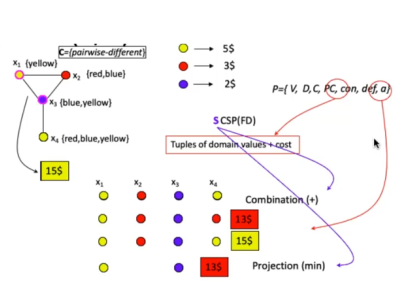
\includegraphics[width=10cm, keepaspectratio]{img/Cap4/scsp.png}
    \caption{Esempio di SCSP su grafo.}
\end{figure}
\\Partiamo riprendendo la definizione di un CSP, esso è definito come P=\{V,D,C,PC,con,def,a\} i quali indicano:
\begin{itemize}
    \item V $=$ insieme delle variabili;
    \item D $=$ insieme dei domini associati alle variabili;
    \item C $=$ insieme di vincoli, definito come l’associazione variabile-vincolo ovvero quali variabili sono coinvolte in quale vincolo;
    \item PC $=$ sono i vincoli primitivi e variano in base al vincolo e al dominio. A seconda del tipo di vincolo che possiamo avere i primitivi possono essere diversi, esempio se lavoro sugli interi esso conterrà vincoli con gli operatori $<,>,=$.
    \\Sostanzialmente esso indica i tipi di vincoli che posso usare se lavoro su un dominio specifico. Inoltre indicano se il vincolo è implicito (tutti i colori diversi) o esplicito (valgono le coppie $<r,g,b>$, $<g,r,b>$, . . . ).
    \item con $=$ funzione che definisce quali variabili sono coinvolte in quale vincolo, essa dato un vincolo restituisce le variabili che sono connesse a questo;
    \item def $=$ funzione che indica quali sono i valori del dominio possibili per una specifica variabile. In un SCSP questa funzione oltre a dire i valori possibili per una variabile deve indicare anche il costo associato a quei valori, nell’esempio in Figura 4.1 se passiamo in input alla funzione def la variabile x1 essa ci ritornerà 19come valori possibile il colore giallo con costo 5. Questa è la differenza con la funzione def di un problema CSP.
    \item a $=$ sottoinsieme di V contenente tutte le variabili interessate nella soluzione del SCSP, ad esempio nel caso del grafo abbiamo che le variabili che ci interessano per la soluzione ottimale sono solo $x_1$ e $x_3$ , non tutte quante.
\end{itemize}
Nell’esempio in Figura 4.1 i vincoli binari sono hard, perché la soluzione richiede per forza che i nodi collegati abbiamo colori diversi sennò si violano i vincoli, mentre i vincoli unari (quelli del costo sul colore) sono soft. Nel caso di un CSP quando utilizziamo un algoritmo di ricerca per trovare una soluzione esso si può fermare alla prima soluzione che trova oppure, se richiesto, le cerca tutte quante. Nel caso di SCSP siamo costretti a trovare tutte le possibili soluzioni in modo da scegliere la
migliore. Normalmente si utilizzano due operazioni per trovare la soluzione ottimale in un SCSP:
\begin{itemize}
    \item \textbf{Combinazione (+):} dove metto insieme tutti gli assegnamenti, combinando i vincoli, quindi si calcola anche il costo totale ad esempio con l’operazione di somma;
    \item \textbf{Proiezione (×):} operazione di scelta della soluzione migliore data dalla combinazione in base al minimo o al massimo del costo.
\end{itemize}
\newpage
\section{Semiring}
Un semiring è una quintupla:
\begin{center}
    $<A, +, x, 0, 1>$
\end{center}
\begin{itemize}
    \item \textbf{A:} l’insieme degli elementi che mi rappresentano i costi, quindi il dominio dei costi, esso può essere l’insieme dei reali oppure un intervallo specifico $[0,1]$
    \item \textbf{+:} operatore di proiezione, usato per fare la scelta fra le soluzioni trovate dalla combinazione, può essere il minimo o massimo. Possiamo definire alcune proprietà:
    \begin{itemize}
        \item \textbf{idempotente:} se faccio a+a dove +=minimo il risultato è sempre a, quando un operatore è idempotente è possibile definire un ordinamento ovvero
        \begin{center}
            $a <= b$ dove b è meglio di a $\Leftarrow \Rightarrow$ $a + b = b$
        \end{center}
    \end{itemize}
    \item \textbf{x:} operatore di combinazione, utilizzato per combinare i vincoli, può essere somma,moltiplicazione etc... dipende dal problema. Possiamo definire alcune proprietà:
    \begin{itemize}
        \item \textbf{commutativa:} si considera il set di vincoli invece delle tuple.
    \end{itemize}
    \item \textbf{0:} rappresenta il valore minimo (peggiore) dell’insieme A, ovvero il bottom sotto il quale non si può andare, per l’intervallo $[0,1]$ è 0;
    \item \textbf{1:} rappresenta il valore massimo (migliore) di A, il top, per l’intervallo $[0,1]$ è 1.
\end{itemize}
Tutti questi che abbiamo visto sono simboli quindi quando si utilizza l’operatore $+$ non si ci si riferisce alla somma ma a un operatore per la proiezione che potrebbe essere minimo o massimo o or.
\subsection{Tipi di Semiring}
\begin{itemize}
    \item \textbf{Probabilistico:} $< R^+ , min, +, +\infty, 0>$ si massimizza la probabilità
    \item \textbf{Weighted:} $<[0, 1] max,x,0,1>$ massimo il costo dato dalla combinazione, dove si fa il prodotto;
    \item \textbf{Fuzzy:} $<[0,1],max,min,0,1>;$
    \item \textbf{Classical:} $<{false,true},$ $\lor$ (OR), $\land$(AND)$, false, true>$
\end{itemize}
\newpage
\subsection{Esempi pratici SCSP: Domanda esame}
Il vincolo in mezzo è binario, se è $< a, a >$ significa "quando X$=$a e Y$=$a" (perchè è tra le variabili x ed y).
\subsubsection{Esempio con probabilistic}
\begin{figure}[htp]
	\centering
    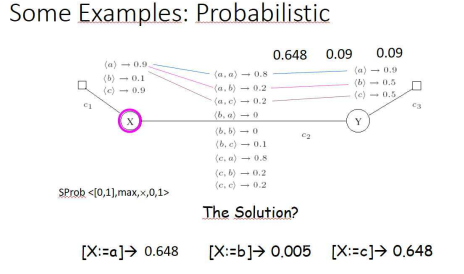
\includegraphics[width=13cm, keepaspectratio]{img/Cap4/probabilistic.png}
\end{figure}
\textbf{Descrizione del semiring:} I valori possibili sono tra 0 ed 1, l’operazione
di proiezione è il Massimo; quella di combinazione è la \textbf{moltiplicazione}; il minimo valore è 0; il massimo valore è 1. 
\\Ci domandiamo: Quanto vale l’assegnamento X $=$ a?
\begin{enumerate}
    \item Dato che l’operazione x di combinazione è la moltiplicazione faccio:
    \begin{enumerate}
        \item 0.9*0.8*0.9 = 0.648
        \item 0.9*0.2*0.5 = 0.09
        \item 0.9*0.2*0.5 = 0.09
    \end{enumerate}
    Per poter inserire 0.648 in x = a dovrei dividere per 0.8 i 3 valori su c2 e 0.9 i tre valori su c3 (secondo me).
    \item Dato che l’operazione + di proiezione in questo caso è Max prendo il massimo di tutti gli elementi trovati e quella sarà la soluzione di quando ad X assegno a.
    Facendo lo stesso ragionamento si calcolano tutte le restanti soluzioni.
\end{enumerate}
\newpage
\subsubsection{Esempio con Fuzzy}
\begin{figure}[htp]
	\centering
    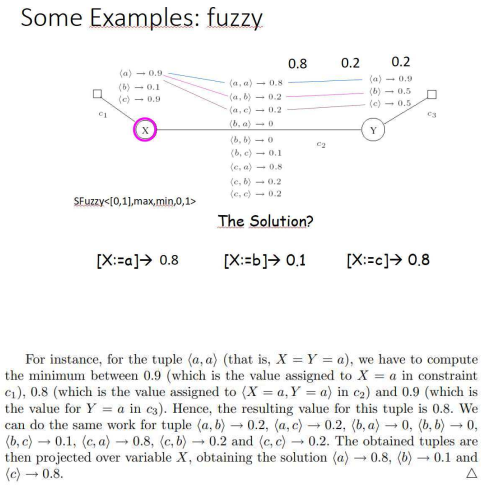
\includegraphics[width=13cm, keepaspectratio]{img/Cap4/fuzzy.png}
\end{figure}
\newpage
\subsubsection{L’aggiunta di vincoli è monotona: peggiora la soluzione}
Questo significa che più aggiungo vincoli e più la soluzione peggiora, più tolgo vincoli più la soluzione mi migliora. Questo perchè più vincoliamo il problema e meno possibilità abbiamo, meno lo vincoliamo e più sono le possibilità. Questo accade nel caso dei vincoli Crisp, nel caso dei vincoli con peso otterremo \textbf{migliori o peggiori} soluzioni.
\subsubsection{Esempio di aggiunta e quindi peggioro}
\begin{figure}[htp]
	\centering
    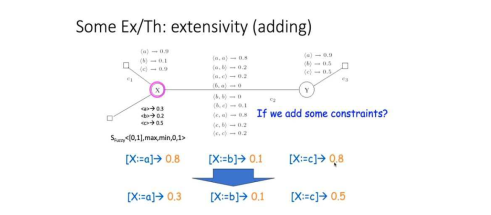
\includegraphics[width=13cm, keepaspectratio]{img/Cap4/worst.png}
\end{figure}
\subsubsection{Esempio di rimozione e quindi miglioro}
\begin{figure}[htp]
	\centering
    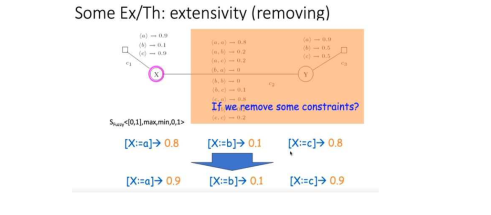
\includegraphics[width=13cm, keepaspectratio]{img/Cap4/better.png}
\end{figure}


